\documentclass[10pt,twoside]{article}
\usepackage[ngerman]{babel}
\usepackage[utf8]{inputenc}
\usepackage{textcomp,gensymb}
\usepackage{longtable}
\usepackage{lscape}
%\usepackage[latin1]{inputenc}
\usepackage{amsmath,thmtools}
\usepackage{siunitx}
\usepackage{enumitem} 
\usepackage{array}
\usepackage{amstext}
\usepackage{amssymb}
\usepackage{stmaryrd}
\usepackage{verbatim}
\usepackage{mathrsfs}
\usepackage{extarrows}
\usepackage[arrow, matrix, curve]{xy}
\usepackage[centering,includeheadfoot,top=25mm, left=40mm, right=25mm, bottom=30mm]{geometry}
\usepackage{gensymb}
\usepackage{graphicx}
\usepackage{framed}
\usepackage[usenames,dvipsnames]{xcolor}
\usepackage{float}
\usepackage{sidecap}
\usepackage{tikz,lipsum,lmodern}
\usepackage{wrapfig} % Allows wrapping text around tables and figures
\usepackage{import}
\usepackage{fancyhdr}
\usepackage{fancybox}
\usepackage{caption}
\usepackage{subcaption}
\usepackage{esint}
\parskip 10pt
\parindent 0pt
\DeclareGraphicsRule{.tif}{png}{.png}{`convert #1 `basename #1 .tif`.png} 
\makeindex
\usepackage[colorlinks,pdfpagelabels,pdfstartview = FitH,bookmarksopen = true,bookmarksnumbered = true,linkcolor = black,plainpages =false,hypertexnames = false,citecolor = black] {hyperref}
\makeatletter
\def\@tocline#1#2#3#4#5#6#7{\relax
  \ifnum #1>\c@tocdepth % then omit
  \else
    \par \addpenalty\@secpenalty\addvspace{#2}%
    \begingroup \hyphenpenalty\@M
    \@ifempty{#4}{%
      \@tempdima\csname r@tocindent\number#1\endcsname\relax
    }{%
      \@tempdima#4\relax
    }%
    \parindent\z@ \leftskip#3\relax \advance\leftskip\@tempdima\relax
    \rightskip\@pnumwidth plus4em \parfillskip-\@pnumwidth
    #5\leavevmode\hskip-\@tempdima
      \ifcase #1
       \or\or \hskip 1em \or \hskip 2em \else \hskip 3em \fi%
      #6\nobreak\relax
    \dotfill\hbox to\@pnumwidth{\@tocpagenum{#7}}\par
    \nobreak
    \endgroup
  \fi}
  \setcounter{tocdepth}{3}
\makeatother
%%%%%%%%%%%%%%%%%%%%%%%RedeclareMathOperator
\makeatletter
\newcommand\RedeclareMathOperator{%
  \@ifstar{\def\rmo@s{m}\rmo@redeclare}{\def\rmo@s{o}\rmo@redeclare}%
}
% this is taken from \renew@command
\newcommand\rmo@redeclare[2]{%
  \begingroup \escapechar\m@ne\xdef\@gtempa{{\string#1}}\endgroup
  \expandafter\@ifundefined\@gtempa
     {\@latex@error{\noexpand#1undefined}\@ehc}%
     \relax
  \expandafter\rmo@declmathop\rmo@s{#1}{#2}}
% This is just \@declmathop without \@ifdefinable
\newcommand\rmo@declmathop[3]{%
  \DeclareRobustCommand{#2}{\qopname\newmcodes@#1{#3}}%
}
\@onlypreamble\RedeclareMathOperator
\makeatother
\renewcommand{\sectionmark}[1]{\markboth{#1}{}}
\lhead{\fancyplain{}{\textit{\leftmark}}}
%%%%%%%%%%%%%%%%%%%%%%%%%%%%%%%%%%%%%%%%%%%%%%%%%%%%%%%%%%%%%%%%%%%%%%%%%%%%%%%%%%Bestimmte Mengen
\newcommand{\C}{\ensuremath{\mathbb{C}}}
\newcommand{\F}{\ensuremath{\mathbb{F}}}
\renewcommand{\P}{\ensuremath{\mathbb{P}}}
\newcommand{\R}{\ensuremath{\mathbb{R}}}
\newcommand{\N}{\ensuremath{\mathbb{N}}}
\newcommand{\Q}{\ensuremath{\mathbb{Q}}}
\newcommand{\Z}{\ensuremath{\mathbb{Z}}}
%%%%%%%%%%%%%%%%%%%%%%%%%%%%%%%%%%%%%%%%%%%%%%%%%%%%%%%%%%%%%%%%%%%%%%%%%%%%%%%%%%Pfeile
\newcommand{\imp}{\Longrightarrow}
\newcommand{\pim}{\Longleftarrow}
\newcommand{\nach}{\longrightarrow}
\newcommand{\hcan}{\longleftarrow}
\newcommand{\nachmenge}{\longmapsto}
\newcommand{\aq}{\Longleftrightarrow}
\newcommand{\surj}{\twoheadrightarrow}
\newcommand{\jrus}{\twoheadleftarrow}
\newcommand{\inj}{\hookrightarrow}
\newcommand{\jni}{\hookleftarrow}
\newcommand{\ximp}{\xLongrightarrow}			%  \xLongrightarrow[\text{unten Text}]{\text{oben Text}} 
																		%%%% Implikation Text oben und untern 
\newcommand{\xpim}{\xLongleftarrow}
\newcommand{\xaq}{\xLeftrightarrow}			%  \xLeftrightarrow[\text{unten Text}]{\text{oben Text}} 
																		%%%% Äquivalenz Text oben und unten
\newcommand{\xnach}{\xlongrightarrow}		
\newcommand{\xhcan}{\xlongleftarrow}										

\renewcommand{\l}{\left\vert}   						%linker Betragsstrich
\renewcommand{\r}{\right\vert}						%rechter Betragsstrich
\newcommand{\ecap}{\cap \ldots \cap}			%Schnit ... Schnitt
\newcommand{\ecup}{\cup \ldots \cup}			%Vereinigung ... Vereinigung
\newcommand{\eplus}{+ \ldots +}					% + ... +
\newcommand{\ekomma}{{,} \ldots {,}}			% , ... ,
\newcommand{\x}{\times}								%  kreuz 
\renewcommand{\d}{~\text{d}}
\renewcommand{\tilde}{\widetilde}
\DeclareMathOperator{\rot}{\text{rot}}
\RedeclareMathOperator{\div}{\text{div}}
\DeclareMathOperator{\laplace}{\vartriangle}
\renewcommand{\epsilon}{\varepsilon}
\newcommand{\qed}{\hfill$\square$\par}
\renewcommand{\bar}{\overline}
%%%%%%%%%%%%%%%%%%%%%%%%%%%%%%%%%%%%%%%%%%%%%%%%%%%%%%%%%%%%%%%%%%%%%%%%%%%%%%%%%%  Hoch minus Zahl
\renewcommand{\1}{^{-1}}				
\renewcommand{\2}{^{-2}}
\newcommand{\3}{^{-3}}
\newcommand{\4}{^{-4}}
\newcommand{\5}{^{-5}}
\newcommand{\6}{^{-6}}
\newcommand{\7}{^{-7}}
\newcommand{\8}{^{-8}}
\newcommand{\9}{^{-9}}
%%%%%%%%%%%%%%%%%%%%%%%%%%%%%%%%%%%%%%%%%%%%%%%%%%%%%%%%%%%%%%%%%%%%%%%%%%%%%%%%%% Definitionsgleich
\newcommand{\define}{\ensuremath{\mathrel{\mathop:}=}} % hübscheres :=, da = zentriert wird relativ zu :
\newcommand{\enifed}{\ensuremath{=\mathrel{\mathop:}}} % hübscheres =:, da = zentriert wird relativ zu :
%%%%%%%%%%%%%%%%%%%%%%%%%%%%%%%%%%%%%%%%%%%%%%%%%%%%%%%%%%%%%%%%%%%%%%%%%%%%%%%%%%Box
\usepackage[most]{tcolorbox}
\definecolor{myColor}{rgb}{0.9,0.9,0.9}		% Farbe für Hintergrund
\definecolor{mycolor}{HTML}{9FB6CD}			% Farbe für Überschriftframe
%%%%%%%%%%%%%%%%%%%%%%%%%%%%%%%%%%%%%%%%%%%%%%%%%%%%%%%%%%%%%%%%%%%%%%%%%%%%%%%%%Abstände
%\, = ein sehr kleiner Abstand
%~ =Leertaste
%\enspace = so breit wie eine Ziffer
%\quad = so breit, wie ein Buchstabe hoch ist
%\qquad = dobbelt so breit wie ein \quad
%\hfill = ein Abstand, der sich von 0 bis unendlich ausdehnen kann
%\hspace{x.ycm} = ein Abstand, der x,y cm lang ist
%%%%%%%%%%%%%%%%%%%%%%%%%%%%%%%%%%%%%%%%%%%%%%%%%%%%%%%%%%%%%%%%%%%%%%%%%%%%%%%%%%XY-Pics
%\begin{figure}[H]
%\begin{center}                     
%\begin{equation*}
%\mbox{%
%$%{\xymatrix{
%
%}
%}$
%}
%\end{equation*}
% \end{center}
% \end{figure}

%\xymatrix{}
%	A  \ar@{.>}[]^"funktion"  B  					gepunkteter Pfeil nach rechts [r] nach links [l]
%	B  \ar2@{<->}[r]^"funktion"  C& 				Äquivalenzpfeil 
%	A  \ar@{->>}[]^"funktion"  B&  					surjektiver Pfeil nach rechts [r] nach links [l]
%	B  \ar@^{(->}[]^"funktion"  &  C 				injektiver Pfeil nach rechts [r] nach links [l]
%	 A  \ar@<2pt>[r]^f  &  B  \ar@<2pt>[l]^g 		oben Pfeil nach B unten Pfeil nach A
%
% Die relativen Richungen sind:
%
%    l - links
%    r - rechts
%    d - unten
%    u - oben
%
%Anstelle der relativen Position kann auch die absolute Position der Ziel-Zelle mittels \ar(·,·) notiert werden - \ar(2,4) läßt den Pfeil zu der Zelle in der zweiten Zeile und vierten Spalte zeigen.
%
%Die Beschriftungen der Pfeile werden an \ar[·] mit folgenden Zeichen angehängt:
%
%    ^ - Beschriftung in Pfeilrichtung links vom Pfeil
%    _ - Beschriftung in Pfeilrichtung auf der rechten Seite
%    | - Beschriftung auf dem Pfeil
%
%So erzeugt \ar[r]^i einen nach rechts zeigenden Pfeil mit darüberstehendem i, 
%während beim nach links weisenden Pfeil \ar[l]^i das i unterhalb des Pfeils steht.
%%%%%%%%%%%%%%%%%%%%%%%%%%%%%%%%%%%%%%%%%%%%%%%%%%%%%%%%%%%%%%%%%%%%%%%%%%%%%%%%%%%%% Satz/Definition/etc Umgebung
\newtcbtheorem[auto counter,number within=section]{satz}%
  {Satz}{enhanced jigsaw,breakable,pad at break*=1mm, colback=cyan!1!white,fonttitle=\bfseries, title=#1}{satz}
\newtcbtheorem[auto counter,number within=section]{defi}%
  {Definition}{enhanced jigsaw,breakable,pad at break*=1mm,colback=green!5,colframe=green!40!black,fonttitle=\bfseries, title=#1}{Definition}
\newtcbtheorem[auto counter,number within=section]{theo}%
  {Theorem}{enhanced jigsaw,breakable,pad at break*=1mm,colback=Bittersweet!5!white,colframe=Bittersweet!95!black,fonttitle=\bfseries, title=#1}{theorem}
\newtcbtheorem[auto counter,number within=section]{koro}%
  {Korollar}{enhanced jigsaw,breakable,pad at break*=1mm,colback=myColor!5!white,colframe=mycolor!75!black,fonttitle=\bfseries, title=#1}{Korollar}
\newtcbtheorem[auto counter,number within=section]{lemma}%
  {Lemma}{enhanced jigsaw,breakable,pad at break*=1mm,colback=myColor!5!white,colframe=mycolor!75!black,fonttitle=\bfseries, title=#1}{Lemma}
\makeatletter
\newcommand{\Beweis}{\textbf{Beweis:}\par}
%%%%%%%%%%%%%%%%%%%%%%%%%%%%%%%%%%%%%%%%%%%%%%%%%%%%%%%%%%%%%%%%%%%%%%%%%%%%%
\usepackage{pgfplots}
\pgfplotsset{compat=1.8}
%%%%%%%%
%\footnote{Fußnotentext} Fussnotentext
%%%%%%%%%%%%%%%%%%%%%%%%%%%%%%
\setlength{\headheight}{15pt}
\pagestyle{fancy}
\fancyhf{}
\fancyhead[LE, RO]{\leftmark}
\fancyhead[RE, LO]{Juliane Ratzsch, Gentian Rrafshi}
\fancyfoot[LE, RO]{\thepage}
\fancyfoot[RE, LO]{\today}
\renewcommand \thesection {\S\arabic{section}}
\renewcommand{\sectionmark}[1]{\markboth{\thesection {}  #1}{}}
\renewcommand{\footrulewidth}{0.4pt}


\begin{document}
\thispagestyle{empty}




\begin{center}
\Large{Universität Stuttgart-Vaihingen}\\
\end{center}


\begin{center}
\Large{Universität Stuttgart \\
Fakultät für Mathematik und Physik \\
Physikalisches Praktikum II}
\end{center}

\vspace*{\fill} 

\begin{center}
\textbf{\begin{Huge}
Helium-Neon-Laser
\end{Huge}}
\end{center}

\vspace*{\fill} 
\begin{flushleft}
\begin{tabular}{llll}
\textbf{Autor:} & & Juliane Ratzsch, MatNr. 2967329 & \\
& & Gentian Rrafshi, MatNr. 2721617 & \\
& & \\
\textbf{Version vom:} & & \today &\\
& & \\
\end{tabular}
\end{flushleft}

\newpage

\thispagestyle{empty}

\tableofcontents

\newpage

\section{Grundlagen}

Grundsätzlich werden für den Aufbau eines Lasers drei funktionale Einheiten benötigt, ein aktives Medium, ein Resonator, und eine Energiepumpe.
Im Zwei-Niveau-System gibt es drei unterschiedliche Übergänge, die Absorption, die spontane Emission , und die stimulierte Emission.
Durch die stimulierte Emission wird ein, zum erregenden Photon, kohärentes Photon erzeugt. Diese kohärenten Photonen werden im Resonator verstärkt.
Betrachtet man viele dieser Systeme, kann man Bilanzgleichungen aufstellen.
Wenn $N_1$ die Anzahl der Systeme im Grundzustand ist, und $N_2$ die der Systeme im angeregten Zustand, gilt:
\begin{equation}
\mathrm{Absorption} \qquad \qquad \frac{dN_1}{dt}= -B_{12} u N_1
\end{equation}
\begin{equation}
\mathrm{spontane \, \, Emission} \qquad \qquad \frac{dN_2}{dt}= - A_{21}  N_2
\end{equation}
\begin{equation}
\mathrm{stimulierte \, \, Emission} \qquad \qquad \frac{dN_2}{dt}= -B_{21} u N_2
\end{equation}
mit den Einsteinkoeffizienten $B_{12}$, $B_{21}$, $A_{21}$ und der Intensität des Strahlungsfeldes u. Aus thermodynamischen Überlegungen folgt $B_{12} = B_{21}$.
Formt man die Gleichungen um nach den sich im Resonator befindenden Photonen n, und berücksichtigt Resonatorverluste, durch die Verlustrate $\beta$ erhält man die Gleichung:

\begin{equation}
\frac{dn}{dt} = B_{12} n (N_2-N_1)-\beta n
\end{equation}

Für den Gleichgewichtszustand sind $N_1$ und $N_2$ konstant. Und es folgt für die Photonen im Resonator:

\begin{equation}
n(t)= N_0 \exp{ \left( \left( B_{21} \left( N_2 - N_1 \right) - \beta \right) t \right) }
\end{equation}

Für Verstärkung braucht man also Besetzungsinversion, $N_2 > N_1$. Das erreicht man durch Pumpen. Im Zwei-Niveau-System ist die Besetzungsinversion durch optisches Pumpen jedoch nicht erreichbar.
Soll optisch gepumpt werden, benötigt man mindestens ein Drei-Niveau-System.

In Abbildung \ref{fig:roehre} ist der schematische Aufbau der He-Ne-Gasröhre zu sehen. 
Der Aufbau entspricht einer Gasentladungsröhre, mit Brewster Fenstern an den Enden, damit das Laserlicht linear polarisiert ist.
Durch das angelegte elektrische Feld, werden He-Atome ionisiert. Die dabei frei gewordenen Elektronen ionisieren weitere Atome oder heben bei geringerer Energie gebundene Elektronen auf ein höheres Energieniveau an.
In Abbildung \ref{fig:termschema} ist das hier interessierende Termschema dargestellt.
He-Atome werden aus dem Grundzustand angeregt auf die Niveaus $2^1S_0$ und $2^3S_1$.
Durch Stöße 2. Art geben die angeregten He-Atome ihre überschüssige Energie ab, und heben Ne-Atome aus dem Grundzustand in den angeregten Zustand 3S oder 2S. Aus diesen Niveaus gibt es strahlende Übergänge, verschiedener Frequenzen. Je nach Aufbau kann der Laser mit diesen Wellenlängen zum Laufen gebracht werden.

\begin{figure}[H]
\centering
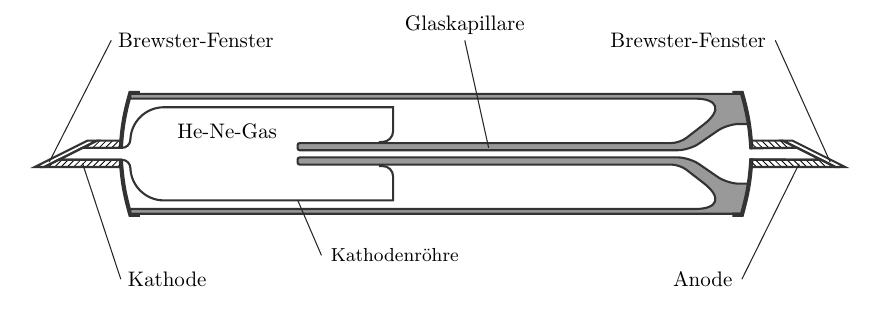
\includegraphics[scale=0.7]{Graphik/roehre.png}  
\caption{Schematische He-Ne-Röhre des Laseraufbaus [5]}
\label{fig:roehre}
\end{figure}

\begin{figure}[H]
\centering
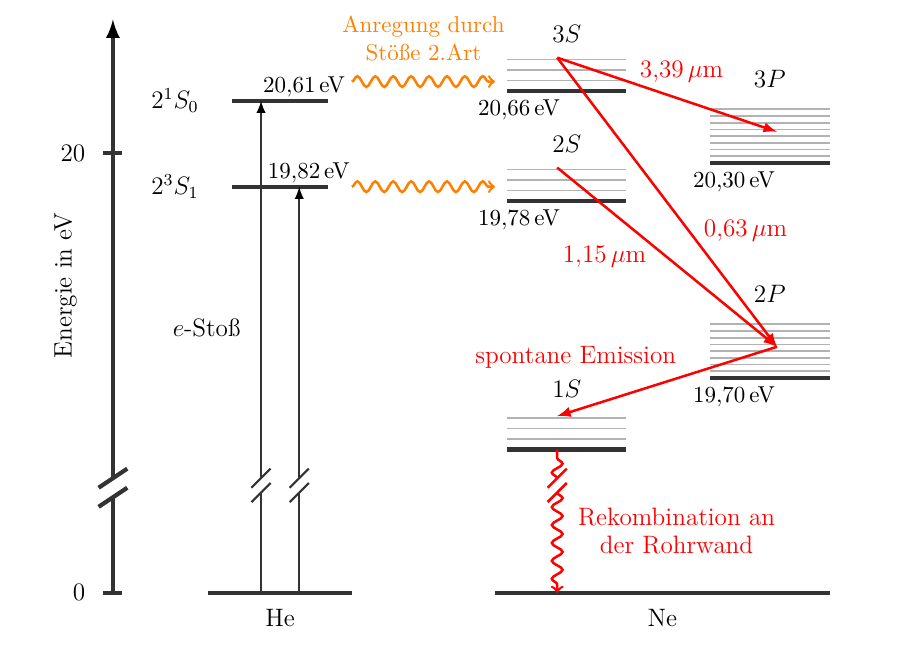
\includegraphics[scale=0.65]{Graphik/termschema.png} 
\caption{Termschema des He-Ne-Lasers [1]}
\label{fig:termschema}
\end{figure}
Für die Untersuchung der TM Moden wird die Helmholtz-Gleichung $\left( \Delta^2 + k^2 \right) \mathbf{E}(x,y,z) = 0 $ gelöst.
Die Gleichung entsteht aus der Wellengleichung durch abseparieren des Zeitanteils.
Vernachlässigt man die Polarisation des Lichts, kann mit einer skalaren Gleichung gearbeitet werden. Es wird eine ebene Welle, die sich in z-Richtung ausbreitet, als Ansatz gewählt.
\begin{equation}
\mathrm{E}(x,y,z)=u(x,y,z)\exp{ikz}
\end{equation}

Einsetzen in die Helmholtzgleichung ergibt:
\begin{equation}
\frac{\partial^2 u}{\partial x^2} + \frac{\partial^2 u}{\partial y^2} + \frac{\partial^2 u}{\partial z^2} - 2ik \frac{\partial u}{\partial z} = 0
\end{equation}

In paraxialer Näherung wird der Term mit der zweiten Ableitung nach z vernachlässigt.
Es folgt die paraxiale Helmholtzgleichung:
\begin{equation}
\frac{\partial^2 u}{\partial x^2} + \frac{\partial^2 u}{\partial y^2} - 2ik \frac{\partial u}{\partial z} = 0
\end{equation}

Die Lösungen der Gleichung sind von der Form:
\begin{equation}
u(x,y,z)=u_0 \frac{w_0}{w(z)} H_m \left( \frac{\sqrt{2}x}{w(z)} \right) H_n \left( \frac{\sqrt{2}y}{w(z)} \right) \exp \left( \frac{-ik(x^2+y^2)}{2q(z)} \right)
\end{equation}

mit den hermiteschen Polynomen $H_m$, dem Strahlradius $w(z)$, der Strahltaille $w_0$, und dem Strahlparameter $q$.

Für $H_m = H_n = 0$ ergibt sich die Grundmode, die auch Gauß-Strahl genannt wird.
Die komplexe Amplitude des elektrischen Feldes lautet

\begin{equation}
E(r,z)= E_0 \frac{w_0}{w(z)} \exp \left( -\left(\frac{r^2}{w(z)} \right) ^2 \right) \exp \left( -ik \frac{r^2}{2R(z)} \right) \exp \left( i( \zeta (z) + kz ) \right) \, \, ,
\end{equation}

mit dem Strahlradius,
\begin{equation}
w(z)= w_0 \sqrt{1+ \left( \frac{z}{z_R} \right) ^2}
\end{equation}
der Rayleigh-Länge,
\begin{equation}
z_R=\frac{\pi w_0^2}{\lambda}
\end{equation}
dem Krümmungsradius,
\begin{equation}
R(z)=z \left( 1 +\left( \frac{z_R}{z} \right) ^2 \right)
\end{equation}
und der Gouy-Phase,
\begin{equation}
\zeta(z) = \arctan \left( \frac{z}{z_R} \right)
\end{equation}

In Abbildung \ref{fig:gauss} ist dieser schematisch dargestellt.


Ein paar höhere Moden sind in Abbildung \ref{fig:tem} dargestellt. Die Ordnung der Hermite-Polynome gibt dabei jeweils die Anzahl der Knoten an.

\begin{figure}
\centering
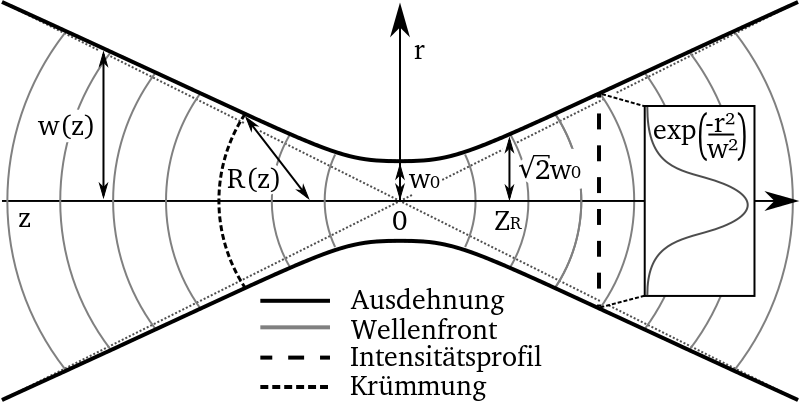
\includegraphics[scale=0.5]{Graphik/gauss_strahl.png} 
\caption{Schematisches Bild eines Gauß-Strahls mit Abmessungsparametern. [3]}
%Bild von א (Aleph), http://commons.wikimedia.org
\label{fig:gauss}
\end{figure}

\begin{figure}
\centering
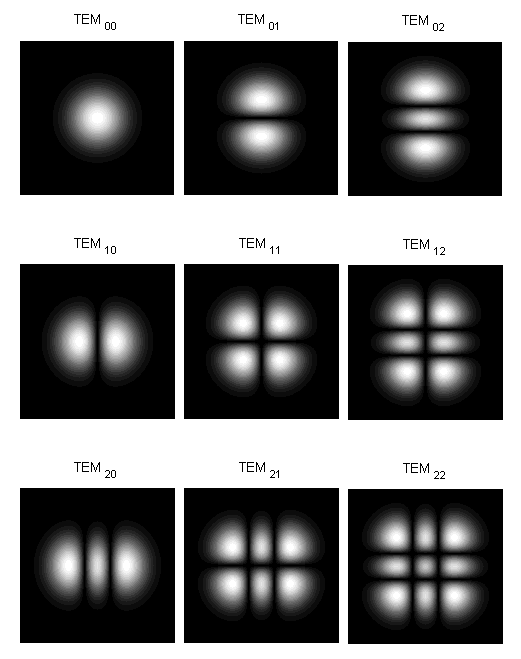
\includegraphics[scale=0.5]{Graphik/tem.png} 
\caption{Intensitätsverteilung verschiedener TEM-Moden [4] }
% https://commons.wikimedia.org/wiki/File:TEMmn.png
\label{fig:tem}
\end{figure}

\subsection{Pre-Lab Exercises}

Abbildung \ref{fig:vier_niveau} zeigt das Termschema eines 4-Niveau Lasers.
Folgende Relationen zwischen den Relaxationszeiten der verschiedenen Übergange maximieren die gewollte Besetzungsinversion zwischen $E_1$ und $E_2$:

- die spontane Emissionsrate von $E_3$ zu $E_2$ soll größer sein als die zu $E_0$.

- die spontane Emissionsrate von $E_1$ zu $E_0$ soll größer sein als die von $E_2$ zu $E_1$.

- Der Übergang von $E_3$ nach $E_2$ soll schneller sein, als der Laserübergang

- Der Übergang von $E_1$ nach $E_0$ soll schneller sein, als der von $E_3$ zu $E_0$

\begin{figure}
\centering
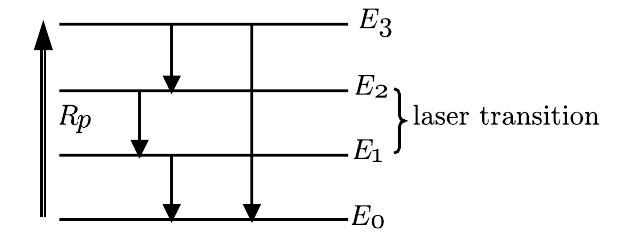
\includegraphics[scale=0.7]{Graphik/vier_niveau.png} 
\caption{Termschema eines 4-Niveau Lasers [2]}
\label{fig:vier_niveau}
\end{figure}

Die Doppler Breite des Lasers beträgt 1,5 GHz. Bei einer Resonatorlänge von 50 cm wird die Anzahl n der longitudinalen Moden geschätzt.
Der Frequenzabstand zweier Moden ist c/2L. Daraus ergibt sich:
$n = \frac{\Delta \nu_{Doppler}}{\delta \nu_{Abstand}} \approx 5$

\newpage
Für den konfokalen Resonator werden im Versuch zwei Spiegel mit einem Krümmumgsradius von 700 mm verwendet, in einem Abstand von 700 mm,
für den sphärischen Resonator zwei Spiegel mit Krümmumgsradius 700 mm, im Abstand von 350 mm.
Und für den hemisphärischen Resonator ein planer Spiegel und einer mit einem Krümmungsradius von 700 mm oder 1000 mm, in einem Abstand kleiner als der Krümmungsradius des zweiten Spiegels.

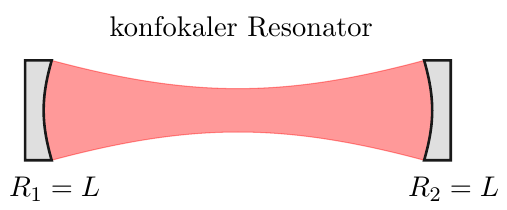
\includegraphics[scale=0.6]{Graphik/konfokal.png} 
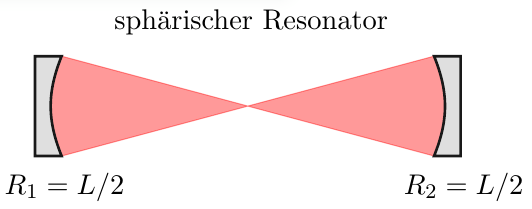
\includegraphics[scale=0.6]{Graphik/sphaerisch.png} 
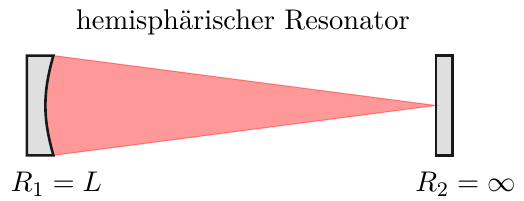
\includegraphics[scale=0.6]{Graphik/hemisphaerisch.png} 

Beim sphärischen Resonator mit großer Resonatorlänge wird erwartet am einfachsten höhere TEM-Moden zu beobachten.


Die Kohärenzlänge wird bestimmt durch die Linienbreite der Frequenz des Lasers. Beim He-Ne-Laser ist der Hauptbeitrag die Doppler-Verbreiterung von etwa 1,5 GHz. Es ergibt sich eine Kohärenzlänge von $l=\frac{c}{\Delta \nu_{D}} \approx 20$ cm.
Mit einem Michelson-Morley-Interferometer kann dies experimentell überprüft werden. Wenn die Wegdifferenz der beiden aufgeteilten Strahlen 20 cm übersteigt, gibt es kein Interferenzmuster mehr, beim Variieren der Wegdifferenz.

\section{Versuchsdurchführung}

Der Aufbau wird so justiert, dass der Laserbetrieb startet.
Mit einem grünen Justage-Laser wird zunächst die Gasröhre so eingestellt, dass der Lichtstrahl beim Durchgang durch die Röhre möglichst wenig verzerrt wird.
Dann werden mit dem grünen Laser die Spiegel justiert, so dass das Licht direkt zurück reflektiert wird.
Mit diesen Einstellungen müssen die Spiegel nur noch minimal justiert werden, damit der Laser startet.

Dann wird für die verschiedenen Resonatortypen das Ausgangssignal gemessen, als Funktion der Resonatorlänge, dann als Funktion der Röhrenposition, und als Funktion des Pumpstroms.

Im nächsten Versuchsteil werden verschiedene TEM-Moden untersucht.
Durch leichtes Verstellen der Spiegel, und durch die Platzierung eines Haares in den Strahlengang werden verschiedene TEM-Moden beobachtet.
Für die Grundmode wird die Divergenz bestimmt. Dazu wird der Strahlradius bei zwei verschiedenen Abständen vom Resonatorende gemessen.

Auch die longitudinalen Moden werden untersucht. Dazu wird das Fabry-Perot-Etalon mit einem Piezo benutzt. Die Einstellungen sind 30-40 Vp-p bei 100 Hz.
Es wird untersucht wie viele Moden zu sehen sind, und wie eine Veränderung der Resonatorlänge die Anzahl verändert.

Um den Laser in den single-mode Betrieb zu bringen, wird in den Strahlengang ein Etalon eingesetzt, und so justiert, dass nur noch eine Mode gemessen wird.

Im letzten Versuchsteil wird ein doppelbrechendes Prisma in den Strahlengang gebracht. Mit einem Spektrometer wird die Wellenlänge des Laserstrahls analysiert. Durch Drehen des Kristalls werden die vier 632,3 nm Moden gesucht. Durch weiteres Drehen wird untersucht, welche weiteren Wellenlängen beobachtet werden können.

%\newpage

\section{Auswertung}

\subsection{Resonatorstabilität}

Im ersten Teil des Versuchs wird das Ausgangssignal als Funktion der Resonatorlänge, als Funktion der Röhrenposition, und als Funktion des Pumpstroms gemessen. Wir verwendeten in diesem Versuch zum einen einen konfokalen und hemisphärischen Resonator.

\subsubsection{Leistung als Funktion der Resontorlänge}
\begin{figure}[H]
\centering
\includegraphics[scale=0.3]{Graphik/Resonatorlange1} 
\caption{Leistung als Funktion der Resonatorlänge für den konfokalen Resonator}
\label{fig:Resonatorlange1}
\end{figure}
\begin{figure}[H]
\centering
\includegraphics[scale=0.3]{Graphik/Resonatorlange2} 
\caption{Leistung als Funktion der Resonatorlänge für den hemisphärischen Resonator}
\label{fig:Resonatorlange2}
\end{figure}
%\begin{figure}[!htb]
%\minipage{0.45\textwidth}
%  \includegraphics[width=\linewidth]{Resonatorlange1}
%  \caption{Leistung als Funktion der Resonatorlänge für den konfokalen Resonator}\label{fig:Resonatorlange1}
%\endminipage\hfill
%\minipage{0.45\textwidth}
%  \includegraphics[width=\linewidth]{Resonatorlange2}
%  \caption{Leistung als Funktion der Resonatorlänge für den hemisphärischen Resonator}\label{fig:Resonatorlange2}
%\endminipage
%\end{figure} \par
Die Abbildungen (\ref{fig:Resonatorlange1}) und (\ref{fig:Resonatorlange2}) zeigen unsere Messerergebnisse für die Leistung als Funktion der Resonatorlänge für einen konfokalen (beide Krümmungsradien R=700\,mm) und einen hemispärischen (ein Krümmungsradius R=700\,mm) Resonator. In folgender Tabelle sind alle nötigen Ergebnisse zusammengefasst, wobei ein Krümmungsradius fix als $r_1=700$\,mm gesetzt wird und die Gehäuselänge des He-Ne-Lasers etwa $39,5$\,cm beträgt:

\begin{tabular}{c||c|c}
~ & konfokaler Resonator & hemispärischer Resonator \\ 
\hline 
Krümmungsradius $r_2$ [mm] & 700\,mm & $\infty$ \\ 
\hline 
theoretische Resonatorlänge L [cm] & $0< L <70$ \& $70< L< 140$ & $0<L<70$ \\ 
\hline 
gemessene Resonatorlänge L [cm] & $39.5<L<110$ & $39.5 < L < 55$ \\ 
\hline 
\end{tabular} 

Der konfokale Resonator hat wie erwartet einen größeren Stabilitätsbereich als der Hemisphärische.
Die gemessene Leistung im konfokalen Resonator sinkt ab einer Resonatorlänge von 110 cm, bei 130 cm ist sie schon stark abgefallen.
Beim hemisphärischen Resonator beginnt die Leistung bereits ab einer Länge von 55 cm zu sinken, schon bei 65 cm startet der Laser nicht mehr.
Die gemessenen Stabilitätsbereiche sind bei beiden Resonatoren etwas geringer als die berechneten, was daran liegen kann, dass die genaue Ausrichtung der einzelne Komponenten des Aufbaus schwer zu erreichen war.

\newpage

\subsubsection{Leistung als Funktion des Resonatorabstandes}

\begin{figure}[H]
\centering
\includegraphics[scale=0.3]{Graphik/Rohr1} 
\caption{Leistung als Funktion des Resonatorabstandes für den konfokalen Resonator}
\label{fig:Rohr1}
\end{figure}

\begin{figure}[H]
\centering
\includegraphics[scale=0.3]{Graphik/Rohr2} 
\caption{Leistung als Funktion des Resonatorabstandes für den hemisphärischen Resonator}
\label{fig:Rohr2}
\end{figure}

%\begin{figure}[!htb]
%\minipage{0.45\textwidth}
%  \includegraphics[width=\linewidth]{Rohr1}
%  \caption{Leistung als Funktion des Resonatorabstandes für den konfokalen Resonator}\label{fig:Rohr1}
%\endminipage\hfill
%\minipage{0.45\textwidth}
%  \includegraphics[width=\linewidth]{Rohr2}
%  \caption{Leistung als Funktion des Resonatorabstandes für den hemisphärischen Resonator}\label{fig:Rohr2}
%\endminipage
%\end{figure} \par

Nun wird die Leistung als Funktion des Resonatorabstandes betrachtet. Aus Abbildung (\ref{fig:Rohr1}) wird ersichtlich, dass beim konfokalen Resonator die Leistung am höchsten ist, wenn die Laserröhre sich mittig zwischen den Resonatorspiegeln befindet, während Abbildung (\ref{fig:Rohr2}) zeigt, dass beim hemisphärischen Resonator die Leistung maximal ist, wenn die Laserröhre möglichst nah am planaren Spiegel ist.

\subsubsection{Leistung als Funktion des Stromes}

\begin{figure}[H]
\centering
\includegraphics[scale=0.27]{Graphik/Strom1} 
\caption{Leistung als Funktion des Stromes für den konfokalen Resonator}
\label{fig:Strom1}
\end{figure}

\begin{figure}[H]
\centering
\includegraphics[scale=0.27]{Graphik/Strom2} 
\caption{Leistung als Funktion des Stromes für den hemisphärischen Resonator}
\label{fig:Strom2}
\end{figure}
%\begin{figure}[!htb]
%\minipage{0.45\textwidth}
%  \includegraphics[width=\linewidth]{Strom1}
%  \caption{Leistung als Funktion des Stromes für den konfokalen Resonator}\label{fig:Strom1}
%\endminipage\hfill
%\minipage{0.45\textwidth}
%  \includegraphics[width=\linewidth]{Strom2}
%  \caption{Leistung als Funktion des Stromes für den hemisphärischen Resonator}\label{fig:Strom2}
%\endminipage
%\end{figure} \par
Bei der Darstellung der Leistung als Funktion des Stromes ist in Abbildung (\ref{fig:Strom1}) zu erkennen, dass ab etwa $5,5$\,mA die Leistung sich bei etwa $4,52$\,mW  sättigt. Beim hemisphärischen sättigt die Leistung ab $6,2$\,mA auf etwa $2.62$\,mW.

\subsection{Untersuchung TEM-Moden}

\begin{figure}[!htb]
\minipage{0.32\textwidth}
  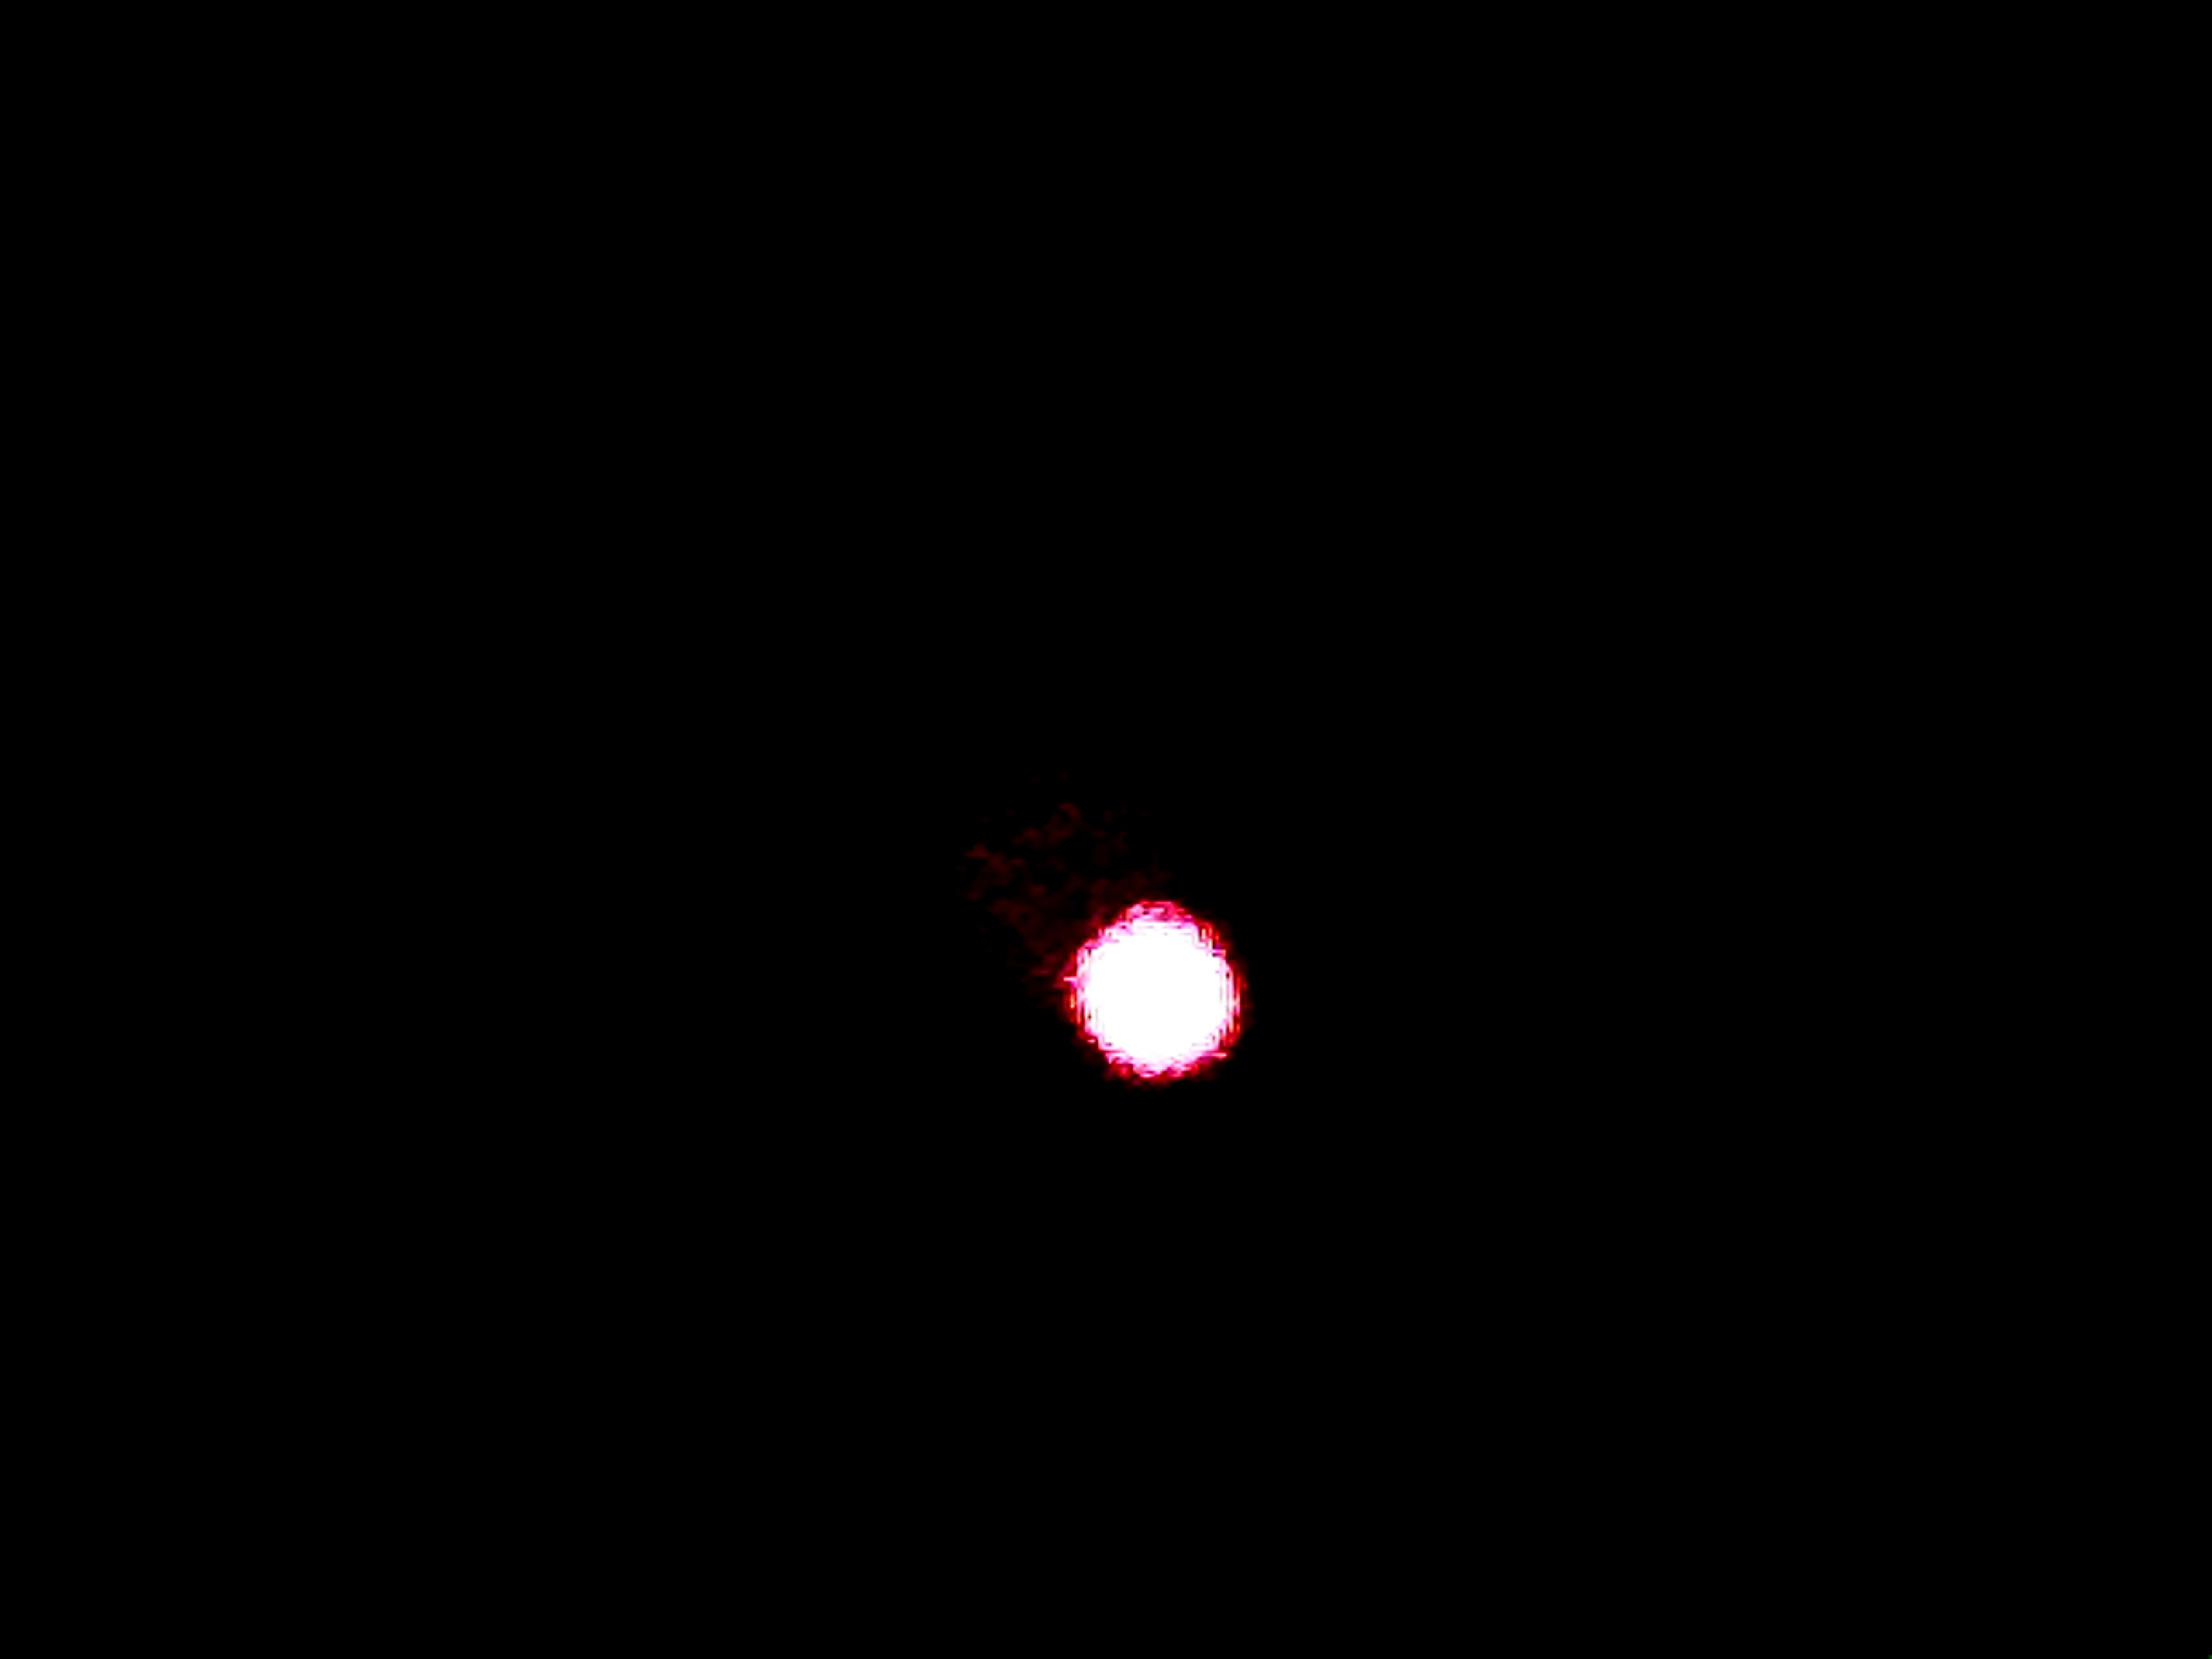
\includegraphics[width=\linewidth]{Graphik/Grund}
\label{fig:Grund}
\endminipage\hfill
\minipage{0.32\textwidth}
  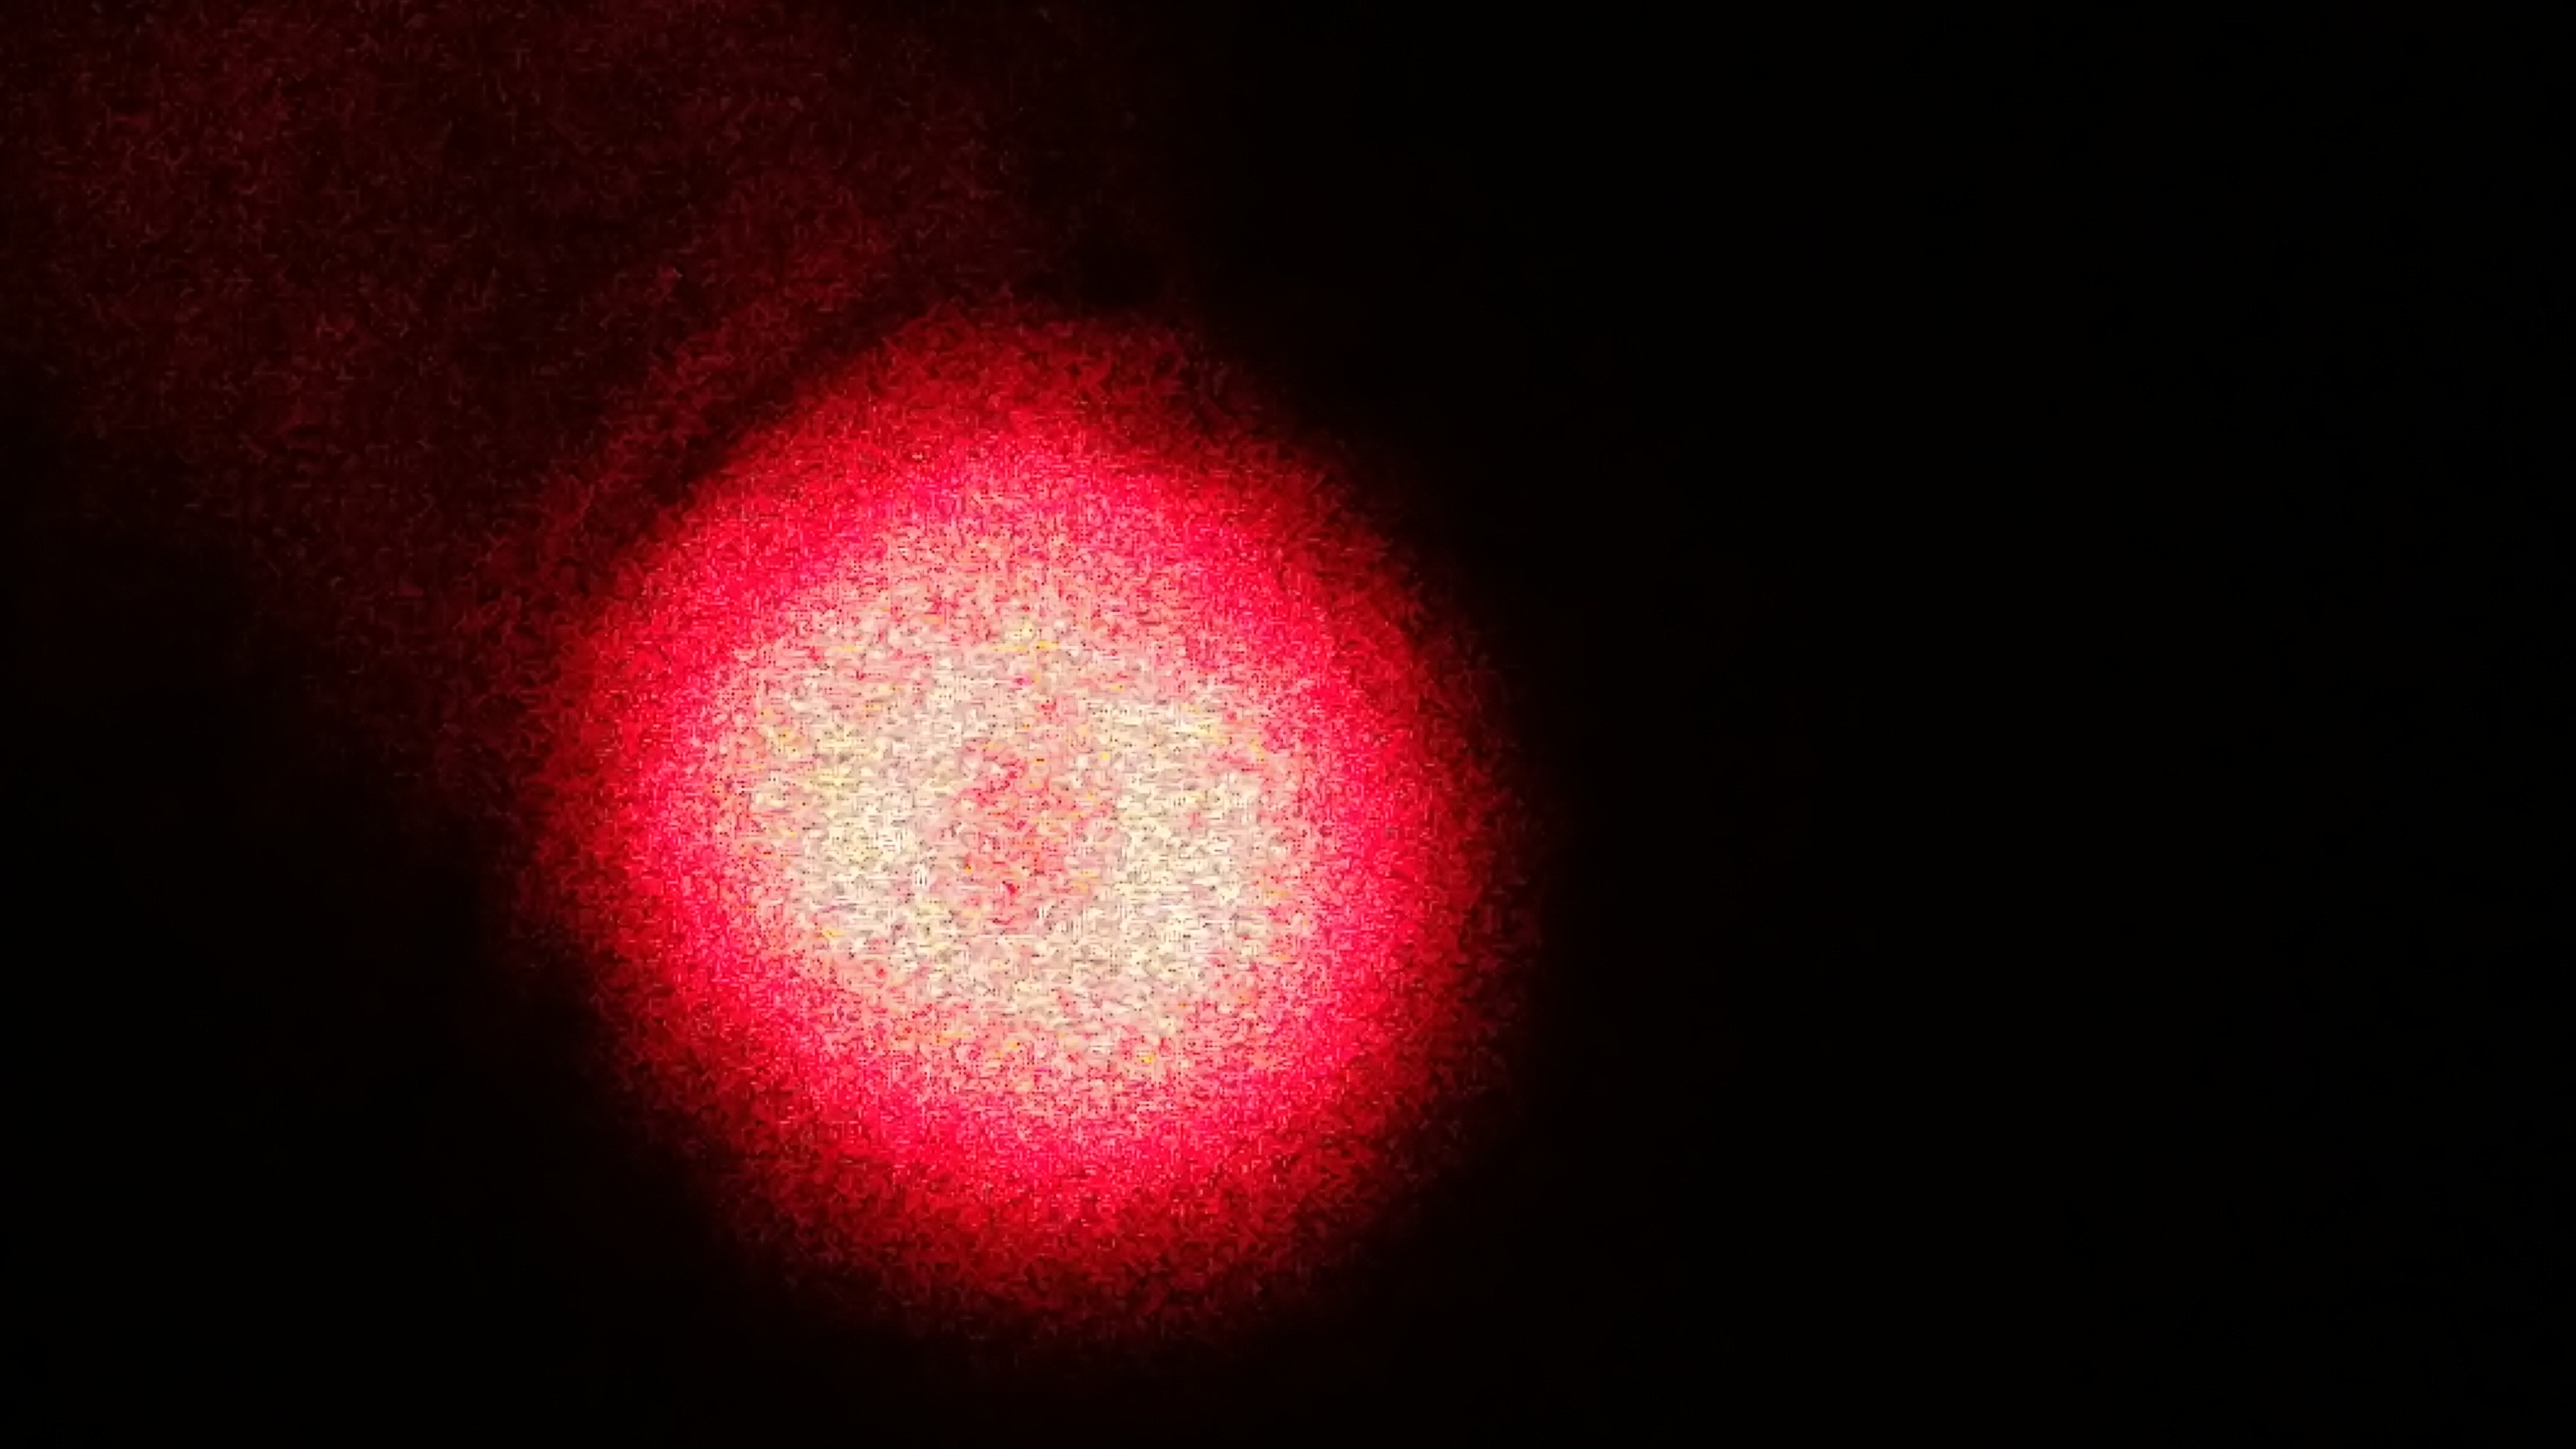
\includegraphics[width=\linewidth]{Graphik/Donut}
\label{fig:Donut}
\endminipage\hfill
\minipage{0.32\textwidth}
  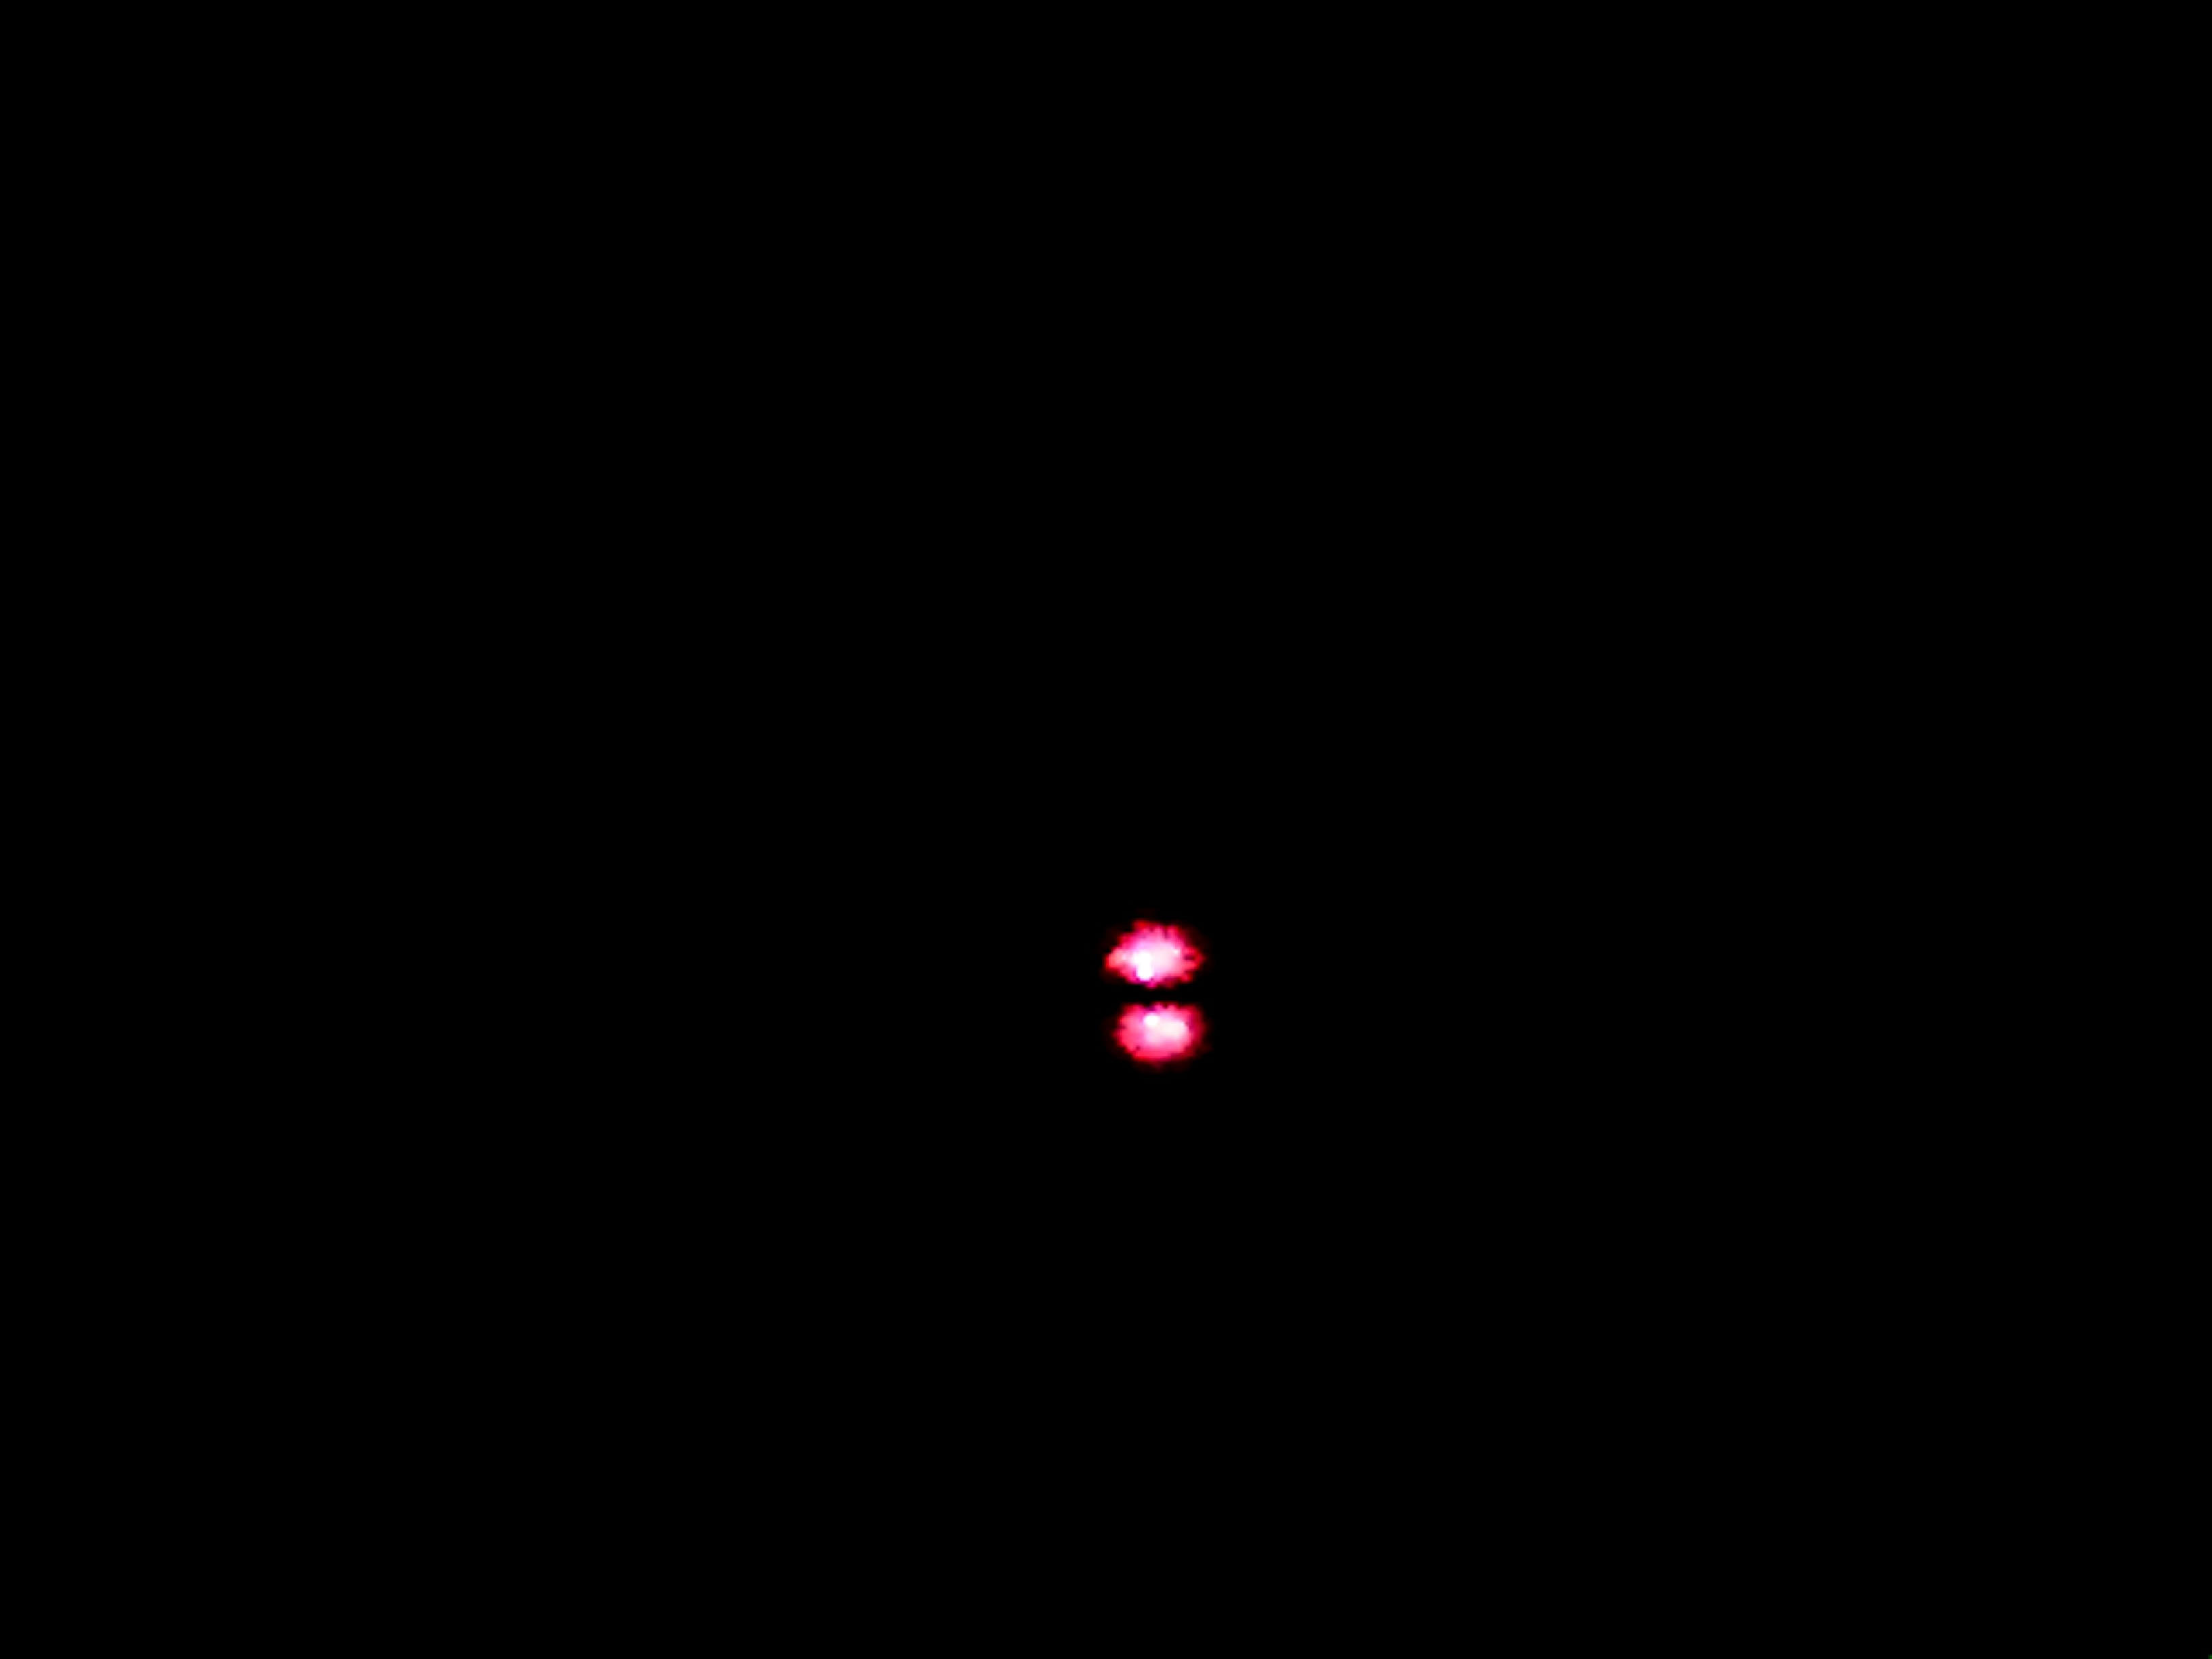
\includegraphics[width=\linewidth]{Graphik/Split}
\label{fig:Split}
\endminipage
\caption{Aufgenommene TEM-Moden mit hilfe eines konfokalen Resonators}
\label{bla}
\end{figure} \par

In diesem Teil des Versuchs sollten wir verschiedene Longitudinale und Transversale Moden erzeugen. Wie in Abbildung (\ref{bla} links) zu sehen ist, haben wir eine Grundmode (TEM$_{00}$), eine TEM$_{10}$ (Abbildung \ref{bla} mitte) und eine TEM$_{01}$ (Abbildung \ref{bla} rechts) erzeugen können. Weiteres war nicht möglich, hierrauf wird in der Fehlerbetrachtung näher eingegangen.

\subsection{Divergenz}

Zur Divergenzbestimmung verwenden wir folgende Formel:
\begin{align*}
\tan(\theta) = \frac{r_2 - r_1}{d}
\end{align*}
Dabei ist $d=115,9$\,cm der Abstand zwischen den gemessen Radien $r_1=0,1$\,cm,$r_2=0,3$\,cm und $\theta$ die Divergenz. Durch Umformen und einsetzen ergibt sich ein Winkel von:
\begin{align*}
\theta \approx 0.1^{\circ}
\end{align*}

\subsection{Longitudinale Moden}

\begin{figure}[!htb]
\minipage{0.32\textwidth}
  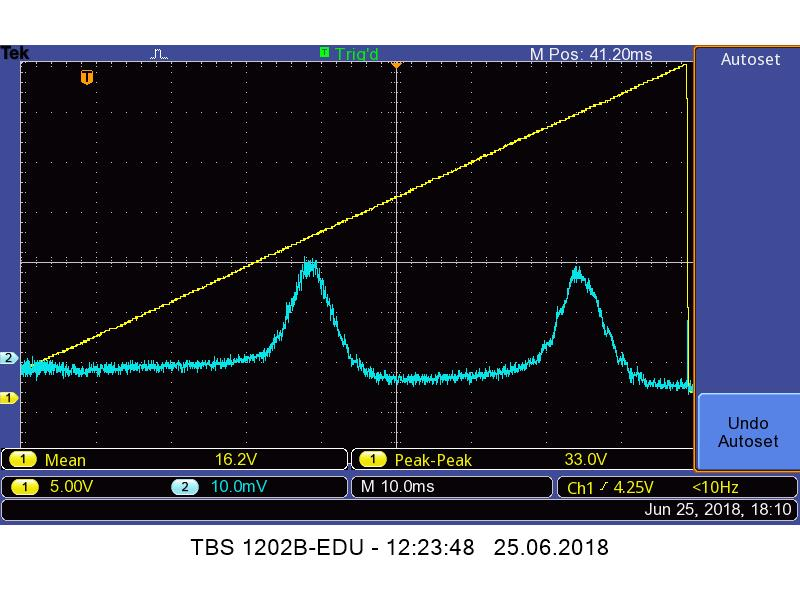
\includegraphics[width=\linewidth]{Graphik/konfokal_45cm}
  \caption{Longitudinale Moden bei 45\,cm Abstand}\label{fig:45}
\endminipage\hfill
\minipage{0.32\textwidth}
  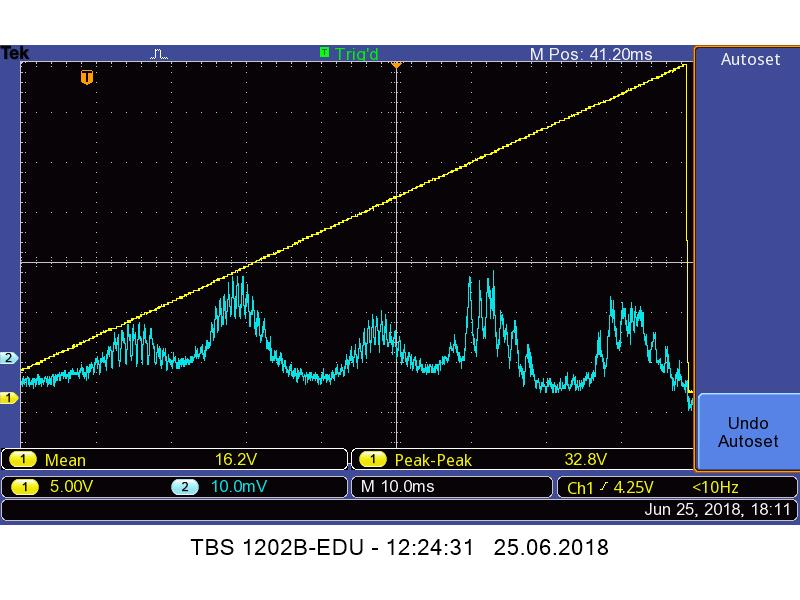
\includegraphics[width=\linewidth]{Graphik/konfokal_55cm}
  \caption{Longitudinale Moden bei 55\,cm Abstand}\label{fig:55}
\endminipage\hfill
\minipage{0.32\textwidth}
  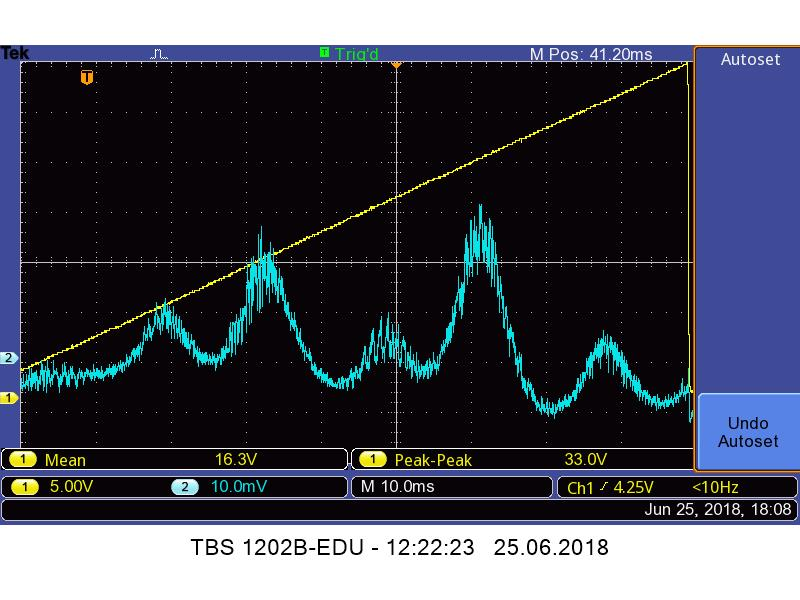
\includegraphics[width=\linewidth]{Graphik/konfokal_65cm}
  \caption{Longitudinale Moden bei 65\,cm Abstand}\label{fig:65}
\endminipage
\end{figure} \par

In diesem Versuchsteil sollten wir uns die longitudinalen Moden anschauen. Laut Prelab-Exercise sollten wir 5 Stück sehen. Bei Abbildung (\ref{fig:45}) sind nur 2 Moden zu erkennen. Erst mit größerer Resonatorlänge sind auch alle 5 zu sehen, wie in Abb.(\ref{fig:55}) und Abb.(\ref{fig:65}) zu sehen ist.   

\subsection{Messung mit Etalon}

\begin{figure}[H]
\centering
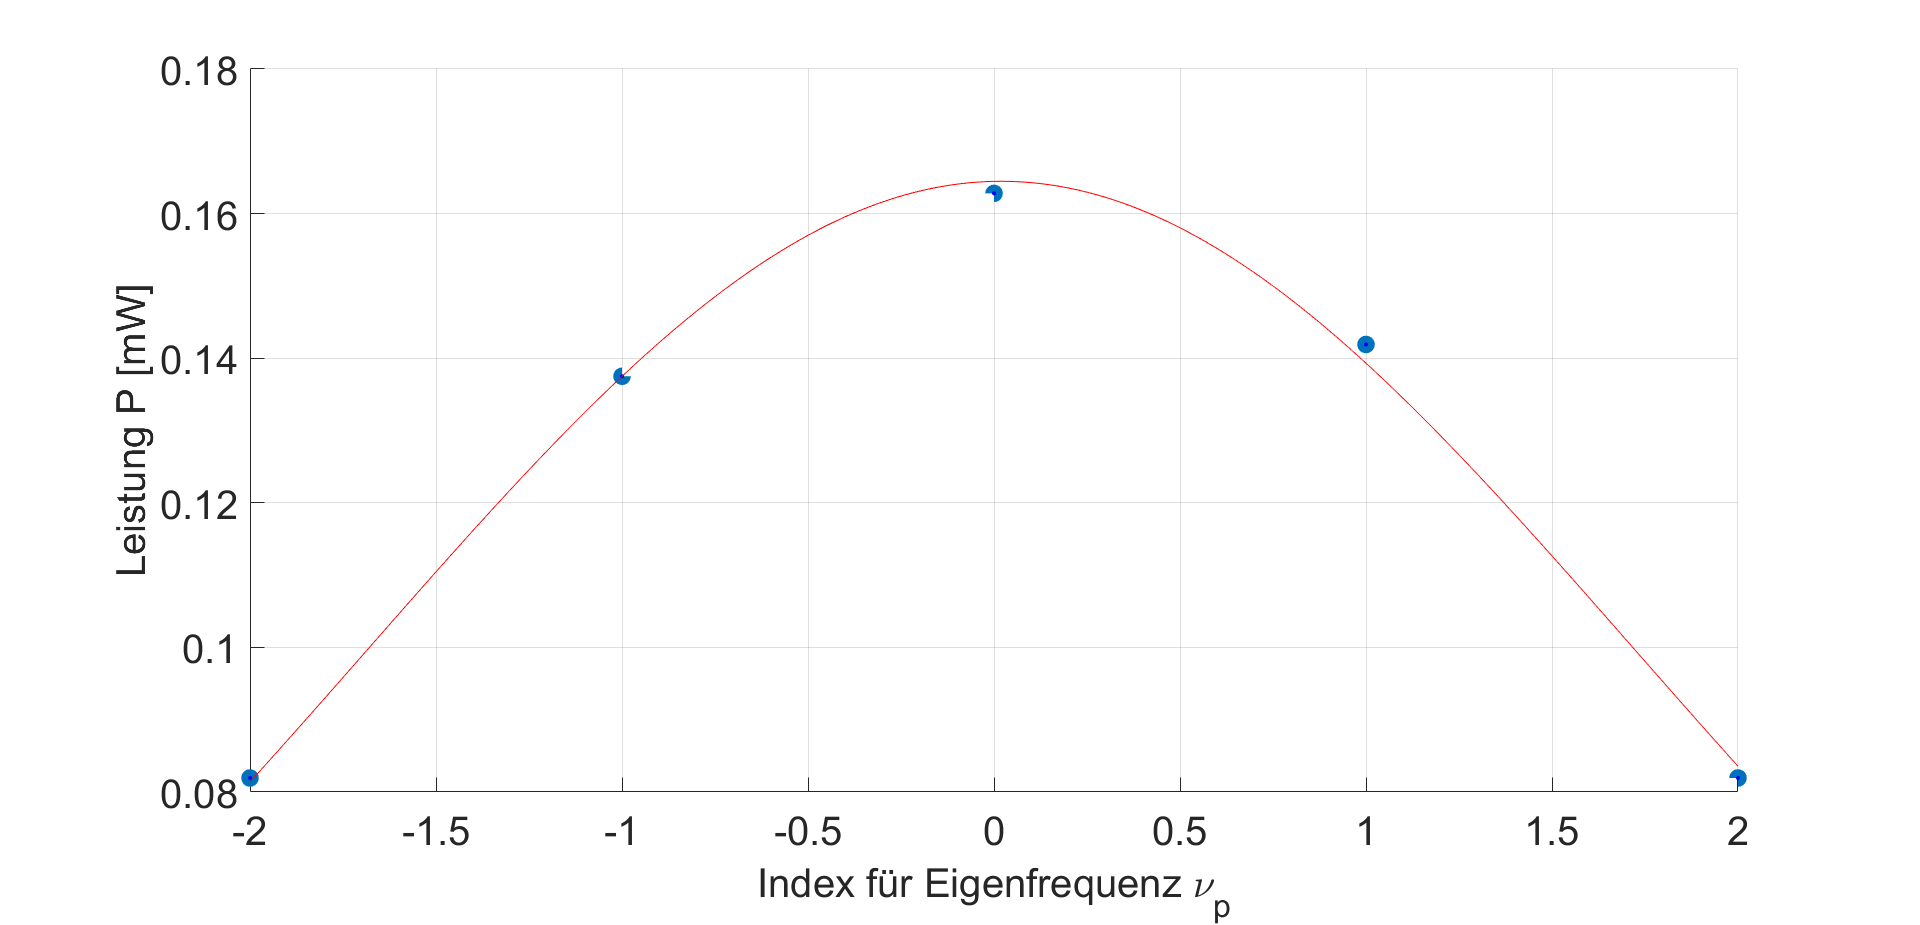
\includegraphics[scale=0.3]{Graphik/Etalon} 
\caption{Leistung der einzelnen longitudinalen Moden. Über diese wurde ein Gaußfit angelegt.}
\label{fig:Etalon}
\end{figure}

Das Fabry-Pérot-Etalon ist ein otpischer Resonator, bestehend aus zwei planparallelen lichtdurchlässigen Quarzglässern, die teilverspiegelt sind. Dadurch erfahren die einfallenden Lichtstrahlen im Resonator konstruktive und destruktive Interferenz. Somit werden bestimmte Wellenlängen selektiert, welche die Resonanzbedingung erfüllen. Daraus folgt, dass die Transmissionsmaxima frequenzabhängig sind und der Frequenzmaximaabstand $\Delta \nu$ wie folgt beschieben werden kann:
\begin{align*}
\Delta \nu = \frac{c}{2\,d\,\left(n^2 -sin(\theta)\right)^{\frac{1}{2}}}
\end{align*}
Hierbei ist $c$ die Lichtgeschwindigkeit, $d$ die Dicke des Etalons, $n$ der Brechungsindex der Quarzplättchen und $\theta$ der Neigungswinkel der Normalen der Resonatorachse. Damit ist durch Rotation ein Einmodenbetrieb möglich. Wie in Abbildung (\ref{fig:Etalon}) zu sehen ist, haben wir 5 Transmissionsmaxima selektieren können. Alle liegen bei der selben Wellenlänge von $\lambda=632.9\,\text{nm}$. Desweiteren wurde ein Gaußfit angelegt, um die Verteilung der Transmissionsmaxima zu untersuchen.


%\newpage

\subsection{Selektion mit dem doppelbrechendem Kristall}

Durch Drehen des doppelbrechenden Kristalls, finden sich verschiedene Positionen bei denen der Laser startet, zwischen diesen bricht der Laserbetrieb zusammen.
Es werden 6 Positionen gefunden, bei denen das Spektrum des Laserlichts aufgenommen wird (Abbildung \ref{fig:prisma}). Die Auflösung des Spektrometers ist nicht optimal für diese Verwendung, es lässt sich aber erkennen, dass die Peaks bei leicht unterschiedlichen Wellenlängen um die 633 nm liegen.

\begin{figure}[H]
\centering
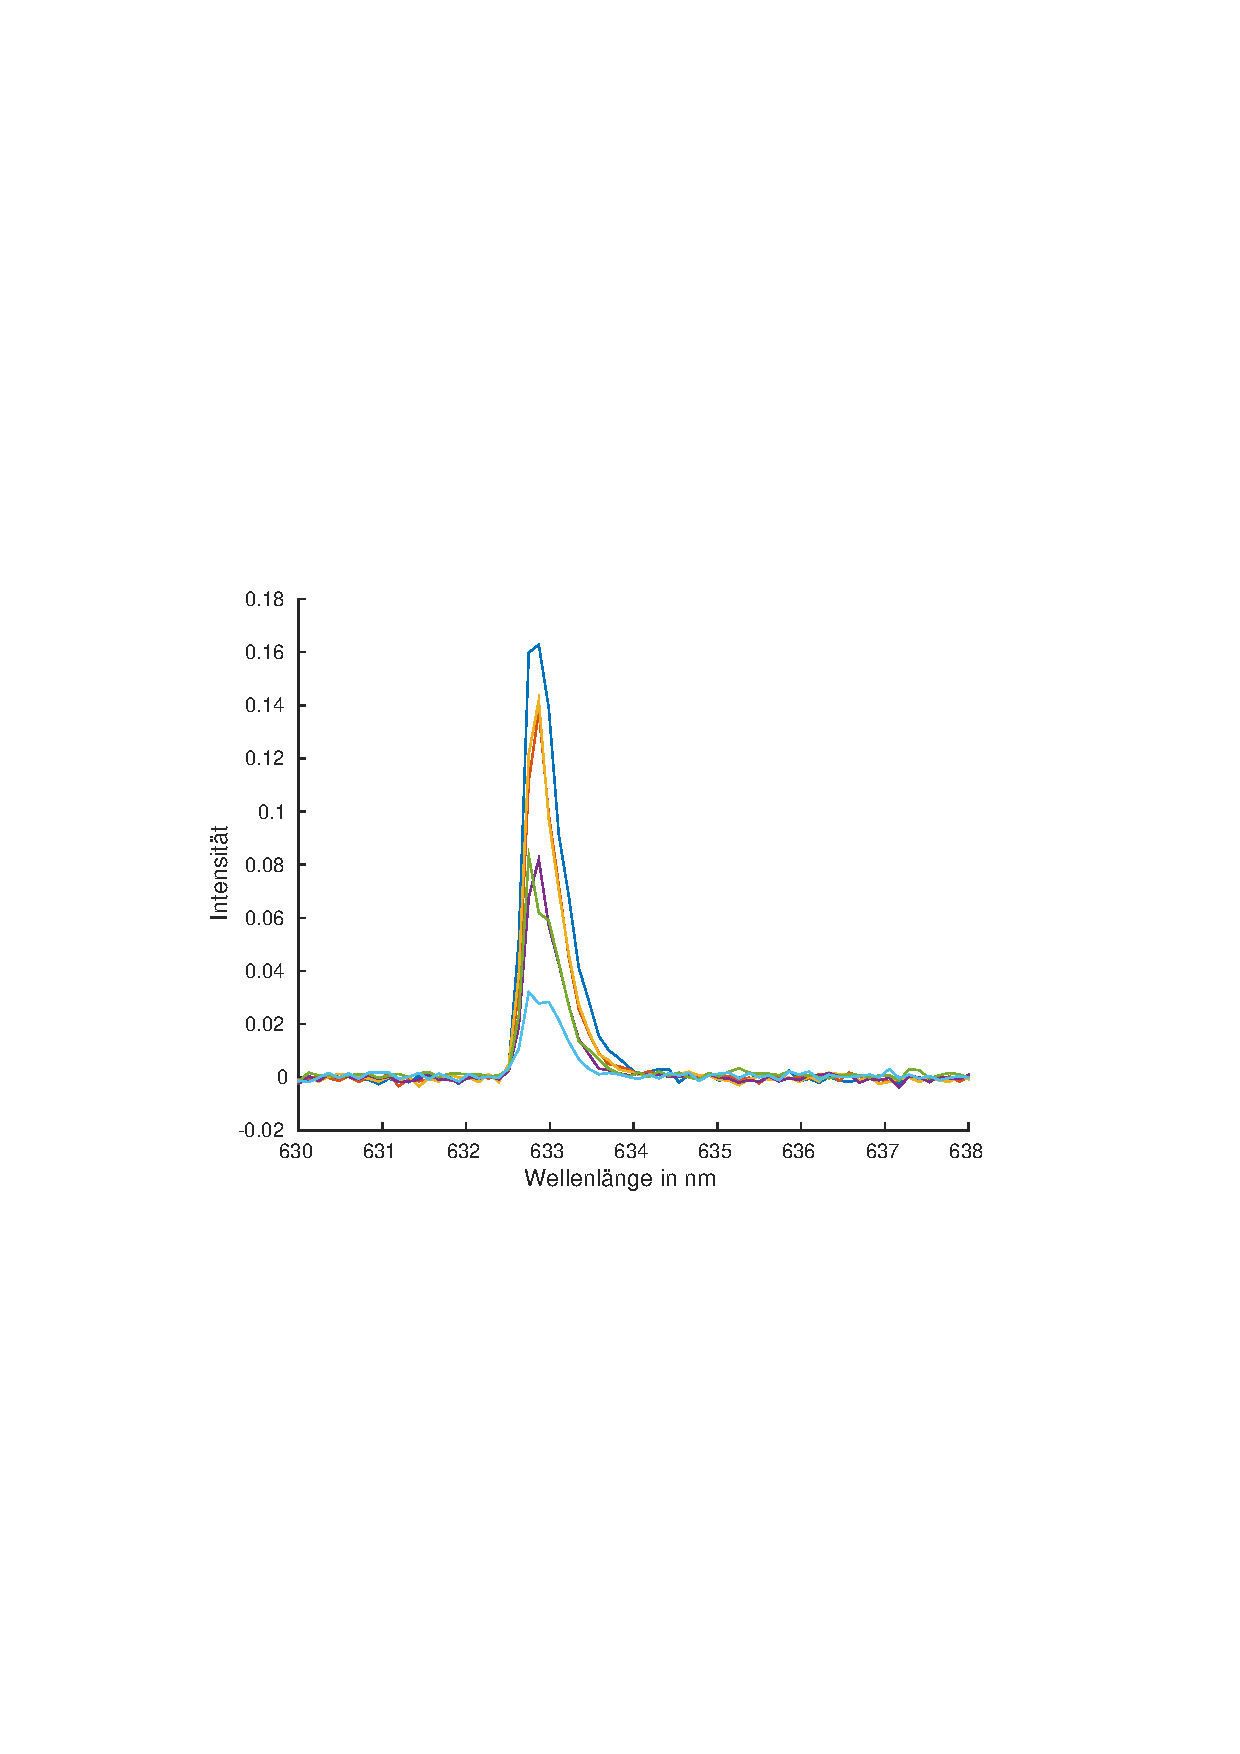
\includegraphics[trim = 1.1in 3.7in 1.1in 3.9in, clip, scale=1]{Graphik/doppelbrechend} 
\caption{Spektrometermessung für verschiedene Drehwinkel des doppelbrechenden Prismas.}
\label{fig:prisma}
\end{figure}

%\begin{figure}[H]
%\centering
%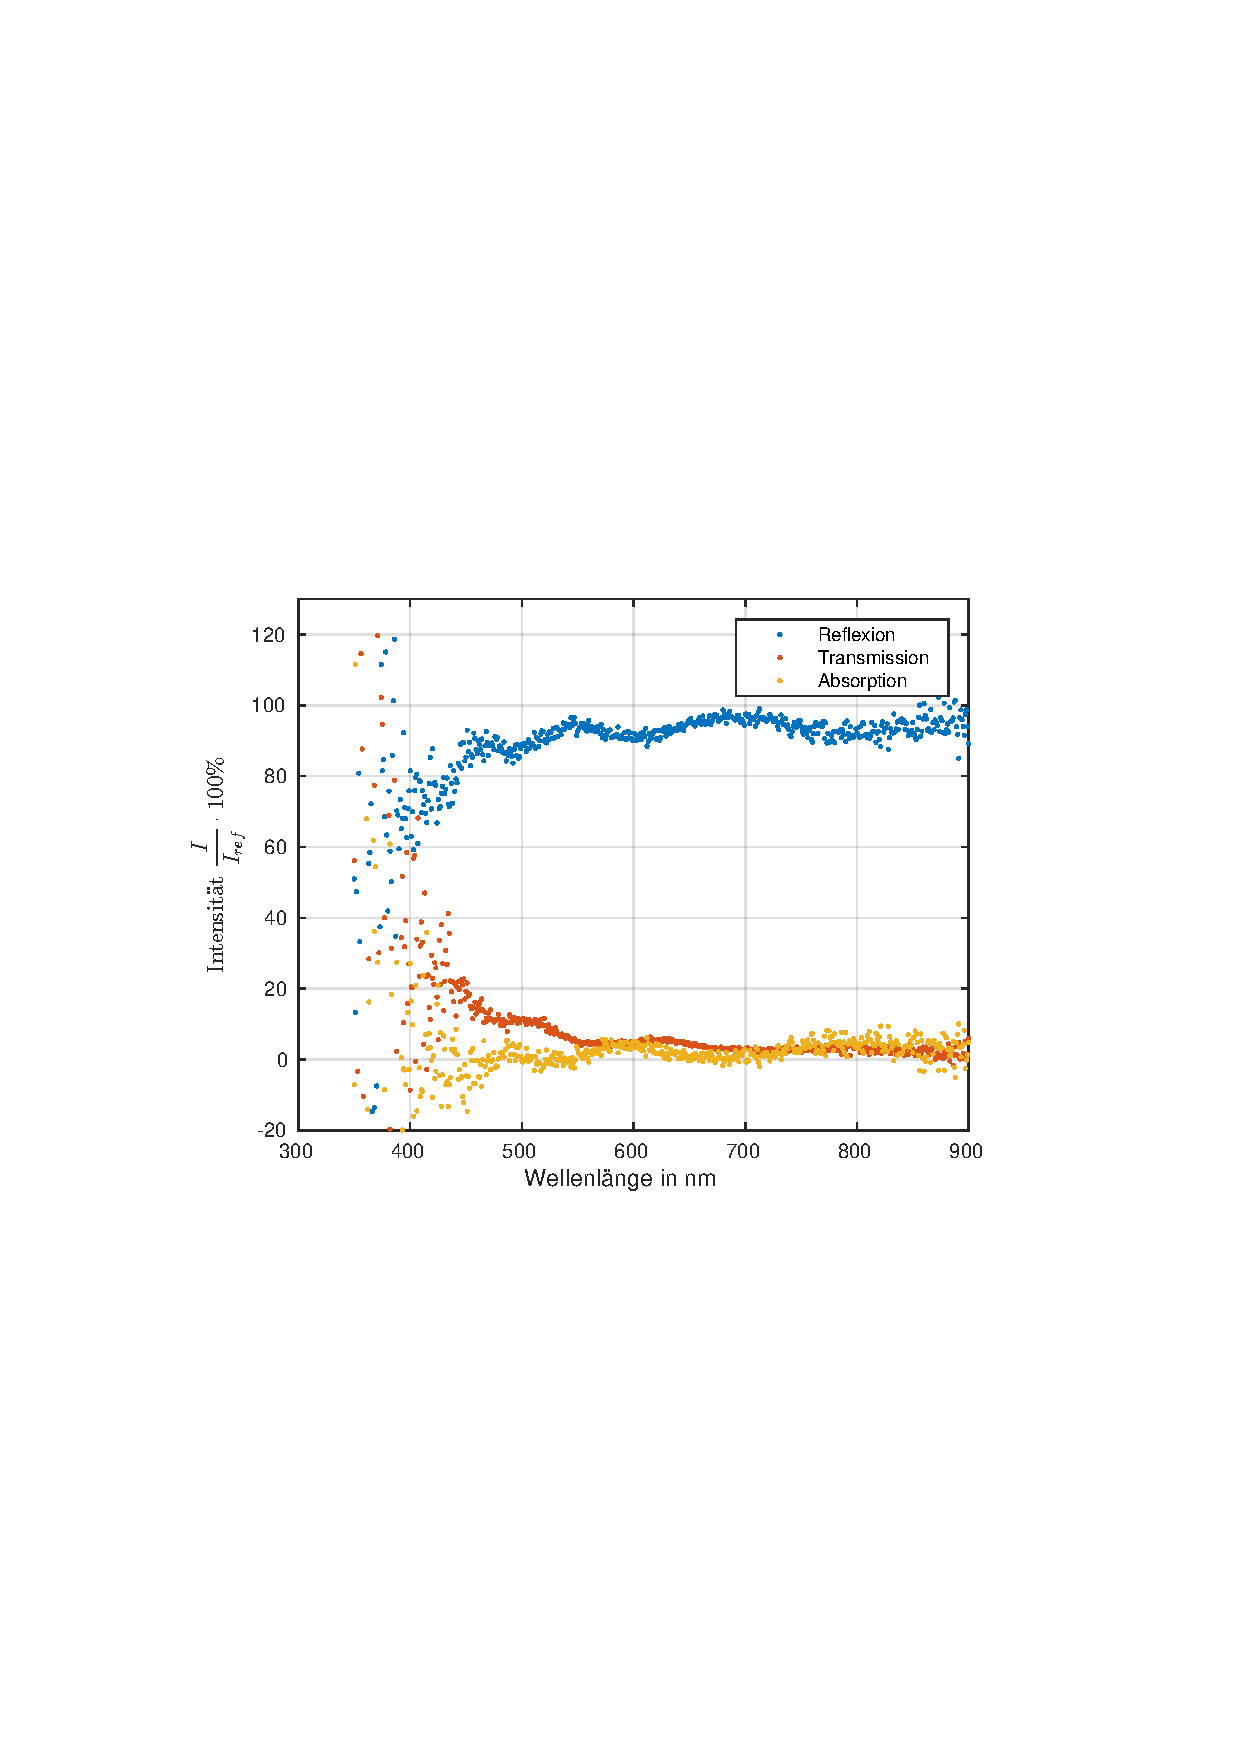
\includegraphics[trim = 1.1in 3.7in 1.1in 3.9in, clip, scale=1]{../Messdaten/Plots/md.pdf} \caption{gemessene Intensitäten der Transmission und Reflexion an einem Zweischichtsystem aus 20 nm Metall und 500 nm Dielektrikum. Die Absorption wurde aus den Daten berechnet.}
%\label{fig:md_500}
%\end{figure}

\section{Fehlerbetrachtung}

Wie schon in der Auswertung angedeutet, war der Versuch technisch sehr empfindlich. So ist es uns nur bei drei TEM-Moden möglich gewesen, eine Fotoaufnahme zu machen. Die anderen Moden sind Aufgrund der schlechten Auflösung nicht möglich gewesen.
Der Laser war auch sehr störanfällig. So war bei kleinsten Bewegungen oder Stöße am Tisch keine Messung möglich.

\section{Zusammenfassung}

Im ersten Teil des Versuchs wurde die Leistung als Funktion der Resonatorlänge, als Funktion der Röhrenposition, und als Funktion des Pumpstroms betrachtet für jeweils einen hemisphärischen und konfokalen Resonator. Als Funktion der Resonatorlänge erfüllten beide die Stabilitätsgleichung $0<(1-\frac{L}{r_1})(1-\frac{L}{r_1})<1$. Betrachtet man die Röhrenposition, so ist das Leistungsmaximum beim konfokalen Resonator genau dann, wenn die Röhre mit dem He-Ne-Gasgemisch sich mittig zu den Resonatoren befindet, beim hemisphärischen Resonator je näher sie sich am planaren Resonator befindet. Als Funktion des Pumpstroms sättigt der hemisphärische Resonator langsamer und bei weniger maximaler Leistung.

Danach wurden TEM-Moden betrachtet, welche in Abbildung (\ref{bla}) zu sehen sind und die Divergenz mit etwa $0.1^{\circ}$ bestimmt.

Bei der Betrachtung der longitudinalen Moden entstehen,mit zunehmendem Abstand, mehr Moden. Es konnten fünf Moden beobachtet werden. Dies stimmt mit unseren Prelab-Exercises überein.

Im letzten Versuchsteil beschäftigten wir uns nochmal mit den longitudinalen Moden. Wir konnten mit dem Fabry-Pérot-Etalon die einzelnen Moden erkennen, welche alle bei der selben Wellenlänge $\lambda=632.9$\,nm lagen und erkannten ebenfalls, dass es sich um 5 gaußverteilte Moden handelt.


\renewcommand{\refname}{\textbf{Literaturverzeichnis}}
\begin{thebibliography}{xxxxxxxxxxxxxxx}

  \bibitem[1]{1}		
\glqq Der Helium-Neon-Laser \grqq ,\\
http://lp.uni-goettingen.de/get/text/1804
 	23.Juli.2018
 	
 	
    	 \bibitem[2]{2}			
Universität Stuttgart (Hrsg.) Physikalisches Praktikum II: Versuchsanleitung. Universität Stuttgart.
2018.

  \bibitem[3]{3}		
\glqq schematischer Gauß-Strahl, Bild von Aleph \grqq ,\\
http://commons.wikimedia.org
 	17.August.2018
	
  \bibitem[4]{4}		
\glqq TEM-Moden \grqq ,\\
https://commons.wikimedia.org/wiki/File:TEMmn.png	
 	17.August.2018		
		 
    	 \bibitem[5]{5}			
\glqq Aufbau eines Versuches für das Fortgeschrittenpraktikum zu den Grundlagen des He-Ne-Lasers \grqq ,
Universität Bremen (Hrsg.) Bacherlorarbeit vorgelegt von Jan Kehlbeck
2018.

%Bild von א (Aleph), http://commons.wikimedia.org		 
		 
% https://commons.wikimedia.org/wiki/File:TEMmn.png		 
		 
\end{thebibliography}

\end{document}